\chapter{Summary and Outlook}
\label{sec:sum}

The main goal of this master project has been to repeat the basic anlaysis steps for the top-quark mass measurement in the $t\bar{t} \rightarrow $ lepton + jets channel for the new 13~TeV data and simulation, while following the  7 and 8~TeV measurements. Therefore a new analyisis framework has been developed. It allows to handle several analysis steps without the need of external code and has a huge flexibility. The workflow of the analysis is illustrated in~\cref{fig:Workflow}.

\begin{figure}
	\center
	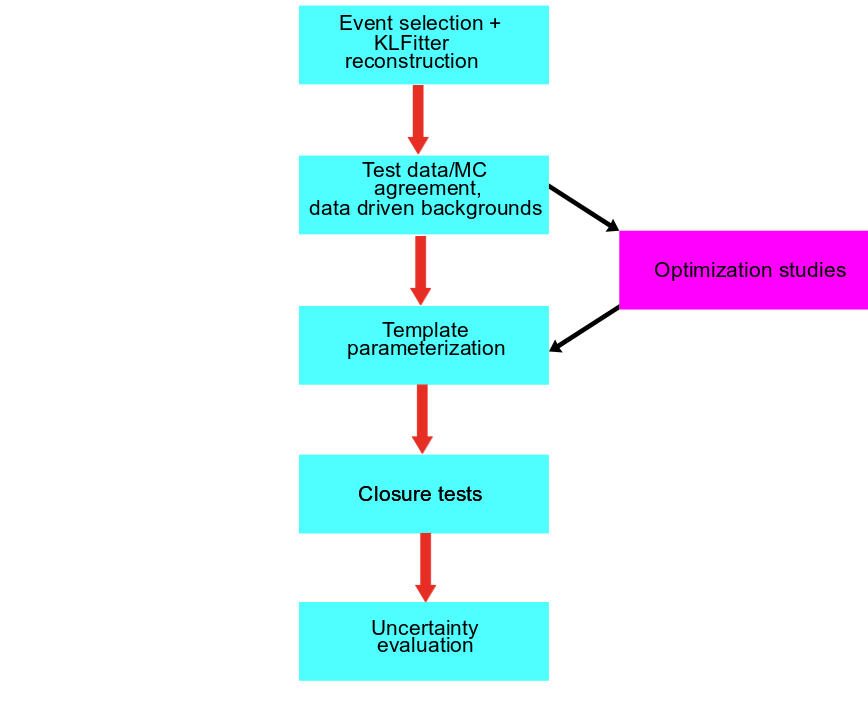
\includegraphics[width=0.6\linewidth]{Pics/Workflow}
	\caption{Workflow of the complete anlaysis.} \label{fig:Workflow}
\end{figure}

 The event selection and event reconstruction have been applied successfully for the 13~TeV data and simulation samples. The selection cuts were adopted to match current analysis recommendations of the ATLAS Top Working Group. The event selection and reconstruction have been performed for events with at least four jets, where at least one jet has to be $b$-tagged, as well as for events with at least four jets, with  at least two $b$-tagged jets.  With the cut on events with at least two $b$-tagged jets a noticeable reduction of the main background, which arises for $W$  + jets events, from 9~\% to 2~\% has been  achieved. The QCD-mulijet background has not been included so far. The corresponding control distributions and  the data/simulation agreement, show in general that there is a common offset in the normalization of the histograms from data and simulation. Furthermore, a disagreement  in the third bin of the number of tagged jets could be observed, as well as a softer description of hadronic top $p_T$ spectrum than predicted. Both of these issues have been already discovered by previous analyses and are under ongoing investigations. Moreover, only statistical uncertainties were included in the control distributions so far, while the observed discrepancies might will be covered by the systematic uncertainties.
 

 The implementation of the template parametrization has been the main part of this thesis. 
The sensitivities of the three estimators ($m_{\text{top}}^{\rm reco}, m_{\text{W}}^{\rm reco}$ and $R_{\text{bq}}^{\rm reco}$) to the top-quark mass and the energy scale factors have been illustrated. In the following, the corresponding distributions have been linearly parametrized in $m_{\text{top}$, JSF and bJSF. In addition,  a simultaneous parametrization has been performed. The linear dependencies have been explicitly shown by linear fits of the fit function parameters in $m_{\text{top}}$, JSF and bJSF. A linear dependence is obseved in general, however there are some deviations in the linearity plots. The information of the single template fit and the linear fits have been used for the initial conditions of the simultaneous template fit of all estimator distributions with different simulated $m_{\text{top}}$, JSF and bJSF. The chosen functional forms describe the distributions well.  The parametrization in  $m_{\text{top}}$, JSF and bJSF of the probability densities  have been used in an unbinned maximum likelihood fit to the simulation.
			
			
 The consistency of the fit has been tested via 250 pseudoexperiments.  Closure tests have been performed of the fit in all three dimensions ($m_{top}$, JSF and bJSF).
 The results of the 1D and 2D fit show only a small bias, while in three dimensions  a larger offset has been found.  The reason for that might be related to the fact that the chosen parametrization does not describe the  estimator distributions well enough. If one considers the linear fits of the fit parameters, one can see that there is a general linear trend, however, there are also noticeable deviations. A similar issue for the 1D and 2D fit has been solved by the optimization of the initial conditions of the simultaneous fit.  Nevertheless, the results of the one-  and two-dimensional fit  demonstrate that the applied method, within the new analysis framework is correct and gave an optimistic outlook that allowed the evaluate of the first systematics. 
 
 The systematic uncertainties have been evaluated via 250 pseudoexpereiments, by varying the corresponding systematic with respect to the nominal sample, or the use of alternative samples instead. The systematics are evaluated for the one-dimensional fit where only $m_{\text{top}}$ is varied, as well as for the two-dimensional fit of  $m_{\text{top}}$ and JSF.  In both cases the dominant systematics are the matrix element generator, the hadronization, the radiation and the jet energy scale.  The total systematics in $m_{\text{top}}$ increases with the higher dimensionality of the fit. The most noticeable increase, which contributes to the higher JES, arises from the JES Flavour Composition which rises from 22~\% to 49~\%. However, there are also systematics, like  for example the radiation or the jet energy resolution, which decrease with the step from 1D to 2D. Furthermore, not all systematics have been included so far, e.g. systematic uncertainties from the PDF and the colour reconnection have been missed. In order make further studies, the uncertainties of all three variables have to be determined.
 At the moment we are assuming a conservative quark-gluon fraction in our sample and therefore observe large flavour related uncertainties. In the future, the uncertainties will be estimated using the quark-gluon fraction that directly corresponds to our selected sample. In previous analyses this has been shown to strongly reduce the corresponding uncertainties.
 
 The focus for the future analysis should be on the optimization of the three-dimensional fit, since the main goal has to be the elimination of the observed bias in the closure tests. 
 Once the 3D fit provides  is successful, the base for whole analysis is  already there and the unbinned maximum likelihood fit can be performed to the data.
 Finally, if the  complete workflow  is flawless, one can start to think about possible 
  optimization studies, e.g. using machine learning techniques, as illustrated in~\cref{fig:Workflow}.
 
 
 


 
  
 
	 


 




 